\section{Sparse matrices, graphs, and tree elimination}

Consider the following illustrative example of how factoring a sparse
matrix can lead to more or less dense factors depending on the order
of elimination.  Putting in $\times$ to indicate a nonzero element, we
have
\[
  \begin{bmatrix}
    \times & \times & \times & \times & \times \\
    \times & \times &        &        &        \\
    \times &        & \times &        &        \\
    \times &        &        & \times &        \\
    \times &        &        &        & \times
  \end{bmatrix} =
  \begin{bmatrix}
    \times &        &        &        &        \\
    \times & \times &        &        &        \\
    \times & \times & \times &        &        \\
    \times & \times & \times & \times &        \\
    \times & \times & \times & \times & \times
  \end{bmatrix}
  \begin{bmatrix}
    \times & \times & \times & \times & \times \\
           & \times & \times & \times & \times \\
           &        & \times & \times & \times \\
           &        &        & \times & \times \\
           &        &        &        & \times
  \end{bmatrix}.
\]
That is, $L$ and $U$ have many more nonzeros than $A$.
These nonzero locations that appear in $L$ and $U$ and not in $A$
are called {\em fill-in}.  On the other hand, if we cyclically
permute the rows and columns of $A$, we have
\[
  \begin{bmatrix}
    \times &        &        &        & \times \\
           & \times &        &        & \times \\
           &        & \times &        & \times \\
           &        &        & \times & \times \\
    \times & \times & \times & \times & \times
  \end{bmatrix} =
  \begin{bmatrix}
    \times &        &        &        & \\
           & \times &        &        & \\
           &        & \times &        & \\
           &        &        & \times & \\
    \times & \times & \times & \times & \times
  \end{bmatrix}
  \begin{bmatrix}
    \times &        &        &        & \times \\
           & \times &        &        & \times \\
           &        & \times &        & \times \\
           &        &        & \times & \times \\
           &        &        &        & \times
  \end{bmatrix}.
\]
That is, the factorization of $PAP^T$ has {\em no} fill-in.

A sparse matrix $A$ can be viewed as an {\em adjacency matrices}
for an associated graphs: make one node for each row,
and connect node $i$ to node $j$ if $A_{ij} \neq 0$.  The graphs
for the two ``arrow'' matrices above are:
%\begin{center}
%\input{lec16fig1.pdf_t}
%\end{center}
\begin{center}
  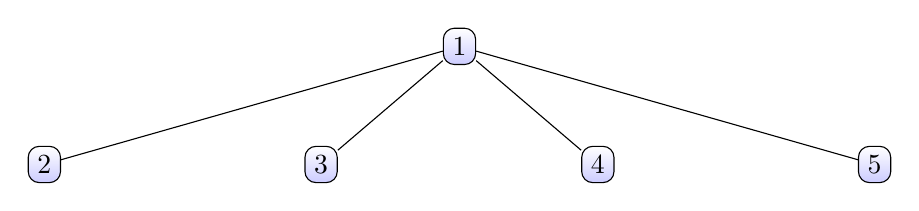
\begin{tikzpicture}[sibling distance=10em,
    every node/.style = {shape=rectangle, rounded corners,
    draw, align=center, top color=white, bottom color=blue!20}]
    \node {1}
      child { node {2} }
      child { node {3} }
      child { node {4} }
      child { node {5} };
  \end{tikzpicture}
  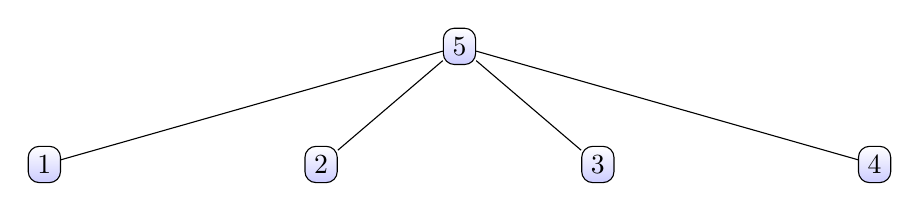
\begin{tikzpicture}[sibling distance=10em,
    every node/.style = {shape=rectangle, rounded corners,
    draw, align=center, top color=white, bottom color=blue!20}]
    \node {5}
      child { node {1} }
      child { node {2} }
      child { node {3} }
      child { node {4} };
  \end{tikzpicture}
\end{center}

These graphs of both our example matrices are {\em trees}, and they
differ only in how the nodes are labeled.  In the original matrix, the
root node is assigned the first label; in the second matrix, the root
node is labeled after all the children.  Clearly, the latter label
order is superior for Gaussian elimination.  This turns out to be a
general fact: if the graph for a (structurally symmetric) sparse
matrix $S$ is a tree, and if the labels are ordered so that each node
appears after any children it may have, then there is no fill-in: that
is, $L$ and $U$ have nonzeros only where $S$ has nonzeros.

Why should we have no fill when factoring a matrix for a tree ordered
from the leaves up?  To answer this, we think about what happens in the
first step of Gaussian elimination.  Our original matrix has the form
\[
  S = \begin{bmatrix} \alpha & w^T \\ v & S_{22} \end{bmatrix}
\]
The first row of $U$ is identical to the first row of $S$,
and the first column of $L$ has the same nonzero structure
as the first column of $A$, so we are fine there.
The only question is about the nonzero structure of the Schur
complement $S_{22}-vw^T/\alpha$.  Note that the update $vw^T/\alpha$
has nonzeros only where $v_i$ and $w_j$ are both nonzero --- that is,
only when nodes $i$ and $j$ are both connected to node $1$.  But node
1 is a leaf node; the only thing it connects to is its parent!  So if
$p$ is the index of the parent of node 1 in the tree, then we only
change the $(p,p)$ entry of the trailing submatrix during the update
--- and we assume that entry is already nonzero.  Thus, the graph
associated with the Schur complement is the same as the graph of the
original matrix, but with one leaf trimmed off.
